
\section{Tools for a Safer Go World}
\label{sec:appr}

%This section describes problems related to \unsafe{} that we identified, as well as information on how to exploit these issues in the wild.
In the following, we present our two novel tools, \toolUsage{} and \toolSA{}, that aid in locating, evaluating and fixing potentially dangerous \unsafe{} usages.




%% ---------------------------------------------------


\subsection{\toolUsage{}: Identification of Unsafe Usage}
\label{sec:appr:toolUsage}

This section presents \toolUsage{}\footnote{\url{https://github.com/jlauinger/go-geiger}}, a novel tool to identify and quantify usages of \unsafe{} in a Go project and in its dependencies. 
%, which is available on GitHub\footnote{\url{https://github.com/jlauinger/go-geiger}}.
Its development was inspired by \textit{cargo geiger}\footnote{\url{https://github.com/rust-secure-code/cargo-geiger}}, a similar tool for detecting unsafe code blocks in Rust programs.

%\subsubsection*{Approach}

Figure~\ref{fig:geiger-architecture} shows an overview of the architecture of \toolUsage{}.
We use the standard parsing infrastructure provided by Go to identify and parse packages including their dependencies based on user input.
%In particular, we use the \textit{packages.Load} function to parse the sources of all packages requested for analysis including their transitive dependencies.
Then, we analyze the AST, %using the standard \textit{ast.Inspect} function.
which enables us to identify different usages of \unsafe{} and their context as described in the next paragraph.
Finally, we arrange the packages requested for analysis and their dependencies in a tree structure, sum up \unsafe{} usages for each package individually, and calculate a cumulative score including dependencies.
We perform a deduplication if the same package is transitively imported more than once.
The \unsafe{} dependency tree, usage counts, as well as identified code snippets, are presented to the user.

%\subsubsection*{Implementation}

We detect all usages of methods and fields from the \textit{unsafe} package, specifically: \textit{Pointer}, \textit{Sizeof}, \textit{Offsetof}, and \textit{Alignof}.
Furthermore, because they often are used in unsafe operations, we also count occurrences of \textit{SliceHeader} \textit{StringHeader} from the \textit{reflect} package, and \textit{uintptr}.
All of these usages are referred to as \unsafe{} usages in this paper.
%The first six \unsafe{} types are detected by finding selector expression nodes with matching field names, while \textit{uintptr} usages are found by inspecting identifier nodes in the AST.
Additionally, we determine the context in which the \unsafe{} usage is found, i.e., 
the type of statement that includes the \unsafe{} usage.
In \toolUsage{} we distinguish between assignments (including definitions of composite literals and return statements), calls to functions, function parameter declarations, general variable definitions, or other not further specified usages.
We determine the context by looking up in the AST starting from the node representing the \unsafe{} usage, and identifying the type of the parent node.
%For example, if the nearest relevant ancestor in the AST is an \textit{AssignStmt} node, then the context is determined as assignment.

%% ---------------------------------------------------



\subsection{\toolSA{}: An Unsafe-focused Linter}
\label{sec:appr:toolSA}

%This section presents \toolSA{}, a novel static code analysis tool to find dangerous \unsafe{} usage patterns that were previously uncaught with existing tools. 
Through the usage of \toolUsage{} in real-world code and our manual analysis in Section~\ref{sec:eval}, we found \unsafe{} code patterns that were not covered by existing linters such as \textit{go vet}. 
To automatically give advice for some of these patterns we designed \toolSA{}\footnote{\url{https://github.com/jlauinger/go-safer}}.
It is meant for assistance during manual audits and also for integration in build chains during development.
%All source code for \toolSA{} is made publicly available\footnote{\url{https://github.com/jlauinger/go-safer}}.
Avoiding the \unsafe{} usage patterns that \toolSA{} detects, prevents the garbage collector race and escape analysis flaw vulnerabilities that we discussed in Section~\ref{sec:appr:vulnerabilites}.

%\subsubsection*{Approach}

\begin{figure}[!t]
    \vspace{2mm}
    \centering
    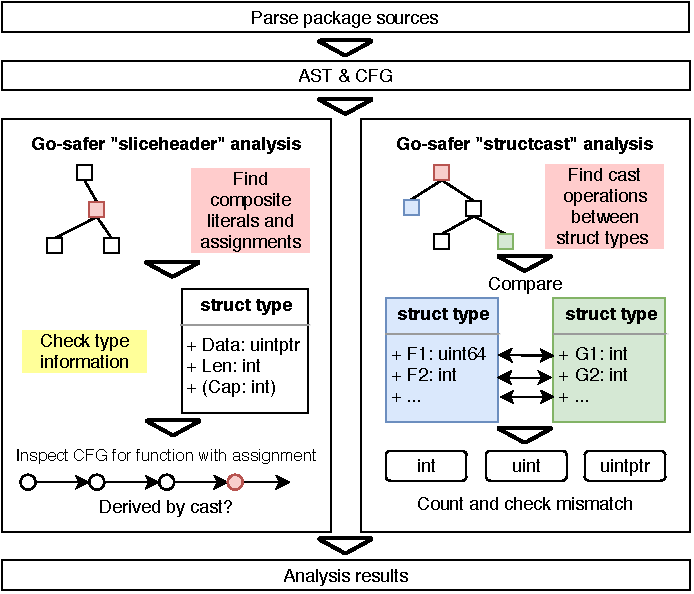
\includegraphics[width=0.48\textwidth]{gfx/figures/go-safer-architecture.pdf}
    %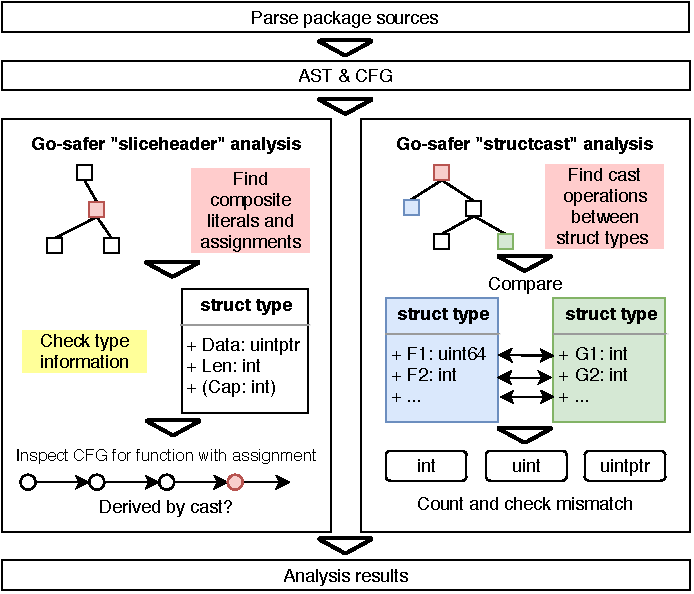
\includegraphics[width=0.45\textwidth]{gfx/figures/go-safer-architecture.pdf}
    \caption{Architecture of \toolSA{} static code analysis tool}
    \label{fig:safer-architecture}
    %\vspace{-14pt}
\end{figure}


Figure~\ref{fig:safer-architecture} shows an overview of the architecture of \toolSA{}.
%It was built on top of the existing infrastructure provided by the \textit{go vet} tool.
First, it uses \textit{go vet} to build a list of packages to be analyzed and parses their sources.
Then, a number of static code analyzers, called \textit{passes}, run.
Our analyses depend on existing passes to acquire the abstract syntax tree (AST) and control flow graph (CFG).
Two separate analyses are run by \toolSA{}: the \textit{sliceheader} and the \textit{structcast} passes. % discovers incorrect string and slice casts as shown in Listing~\ref{lst:string-to-bytes}.
%The \textit{structcast} pass finds unsafe casts between different struct types that include architecture-dependent field sizes and, therefore, might create a security risk when ported to other platforms.
%Describing potential exploit vectors for this second type of problem is beyond the scope of this paper, thus, we added an example of this to the public repository\textsuperscript{\ref{fn:poc}} mentioned in the last section.

%\subsubsection*{Implementation}

The \textit{sliceheader} pass discovers incorrect string and slice casts as shown in Listing~\ref{lst:string-to-bytes}.
It finds composite literals and assignments in the AST.
Then, for each it checks whether the type of the %literal or assignment 
receiver is \textit{reflect.StringHeader}, \textit{reflect.SliceHeader}, or some derived type with the same signature.
For assignments, the analysis pass then finds the last node in the CFG where the receiver object's value is defined, and checks if it is derived correctly by casting a string/slice.
If we can not infer with certainty that the assignment receiver object was created by a cast, then \toolSA{} issues a warning.

The \textit{structcast} pass discovers instances of in-place casts between different struct types that include architecture-dependent field sizes. 
This can create a security risk when ported to other platforms because \unsafe{} casts can lead to misaligned fields, and thus, memory access outside a value's bounds on some platforms, allowing the same exploit vectors as a buffer overflow does.
The pass finds struct cast instances that involve \textit{unsafe.Pointer} in the AST.
Then, it compares the struct types and checks if they contain an unequal amount of fields with types \textit{int}, \textit{uint}, or \textit{uintptr}, which are the architecture-dependent types supported by Go.
If the numbers do not match, \toolSA{} issues a warning.

